\documentclass{article}
\usepackage[utf8]{inputenc}
\usepackage[T1]{fontenc}
\usepackage{pdfpages}

\begin{document}

\textbf{/F60/} \\
\textbf{Prozess:} Gemeinsames Losgehen \\
\textbf{Ziel:} Gruppe geht gemeinsam los \\
\textbf{Kategorie:} primär \\
\textbf{Vorbedingung:} Alle Benutzer sind Mitglieder der selben Gruppe \\
\textbf{Nachbedingung (Erfolg):} Mehrere Gruppenmitglieder gehen als Gruppe los\\
\textbf{Nachbedingung (Fehlschlag):} Die Gruppenmitglieder gehen nicht gemeinsam los\\
\textbf{Akteure:} Gruppenmitglieder \\
% TODO Go-Button schon zu GUI-/Implementierungs-spezifisch?
\textbf{Auslösendes Ereignis:} Ein Gruppenmitglied drückt auf den "Go"-Button\\
\textbf{Beschreibung:}
\begin{enumerate}
\setlength{\itemsep}{0pt}
\item Ein Gruppenmitglied drückt auf den "Go"-Button.
\item Der Standort der Person wird zum Server übertragen.
\item Der Standort wird zu allen Gruppenmitgliedern übertragen.
\item Alle anderen Gruppenmitglieder bekommen eine Benachrichtigung.
\item Auf einer Karte wird die Position der Gruppenmitglieder angezeigt.
\end{enumerate}

%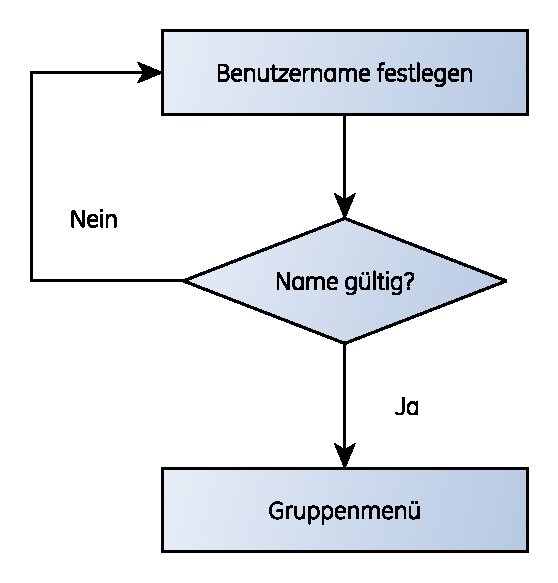
\includegraphics[scale=0.8]{erstmaliges-starten.pdf}

\end{document}
